\section{结果报道}
\subsection{截面结果}
以$\pt$、$y$为函数的$\pp$对撞直接产生的$\psitwos$和由$b$强子衰变产生的$\psitwos$微分产生截面分布如图~\ref{tab:results_prompt}和图~\ref{tab:results_fromb}所示。
相应的数值结果我们放在附录~\ref{sec:ResultTables}的表~\ref{tab:results_prompt}和表~\ref{tab:results_fromb}之中。
%%%%%%%%%%%%%%%%%%%%%%%%%%%%%%%%%%%%%%%%%%%%%%%%%%%%%%%%%%%
\begin{figure}[!tbp]
\centering
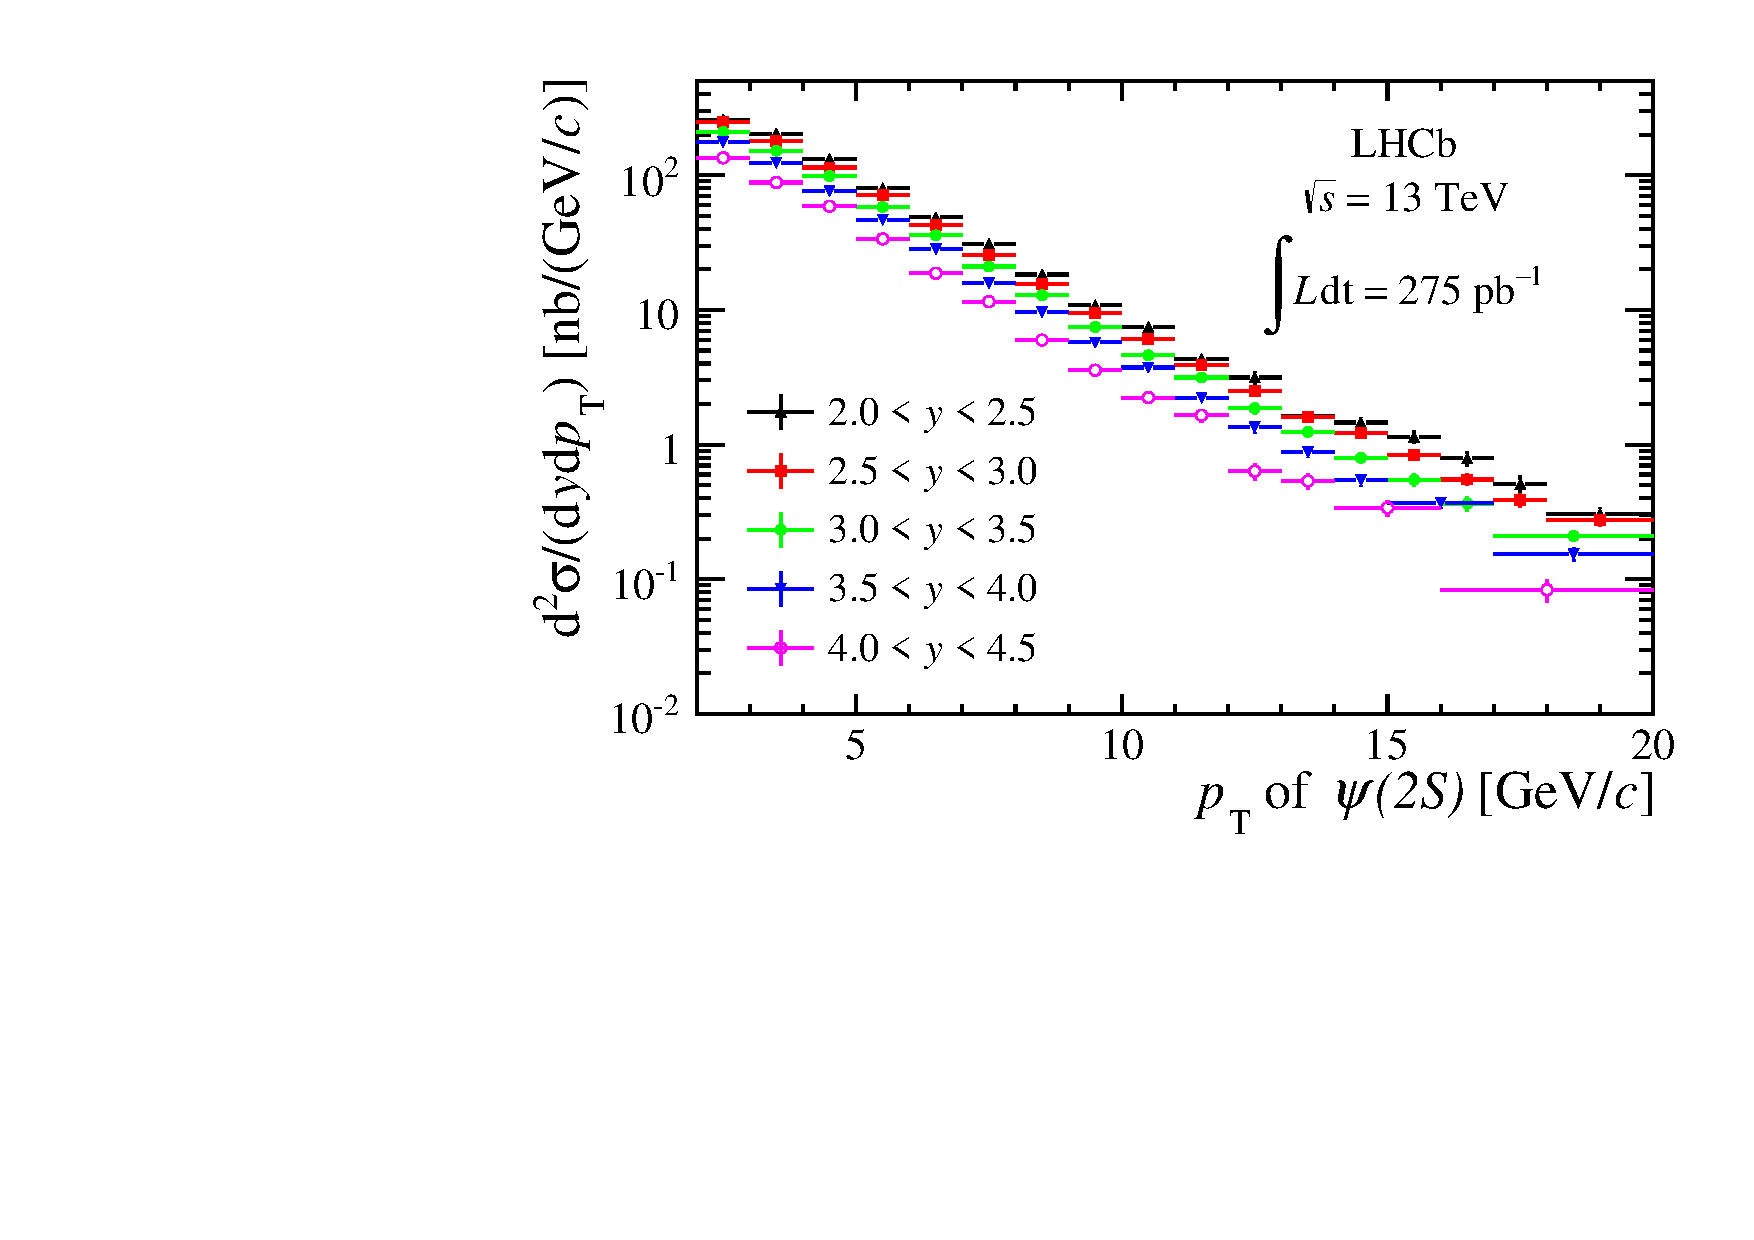
\includegraphics[width=0.9\textwidth]{chap3_result_prompt}
\caption{$\pp$对撞直接产生的$\psitwos$的双微分产生截面分布图。}
\label{fig:results_prompt}
\end{figure}
%%%%%%%%%%%%%%%%%%%%%%%%%%%%%%%%%%%%%%%%%%%%%%%%%%%%%%%%%%%
%%%%%%%%%%%%%%%%%%%%%%%%%%%%%%%%%%%%%%%%%%%%%%%%%%%%%%%%%%%
\begin{figure}[!tbp]
\centering
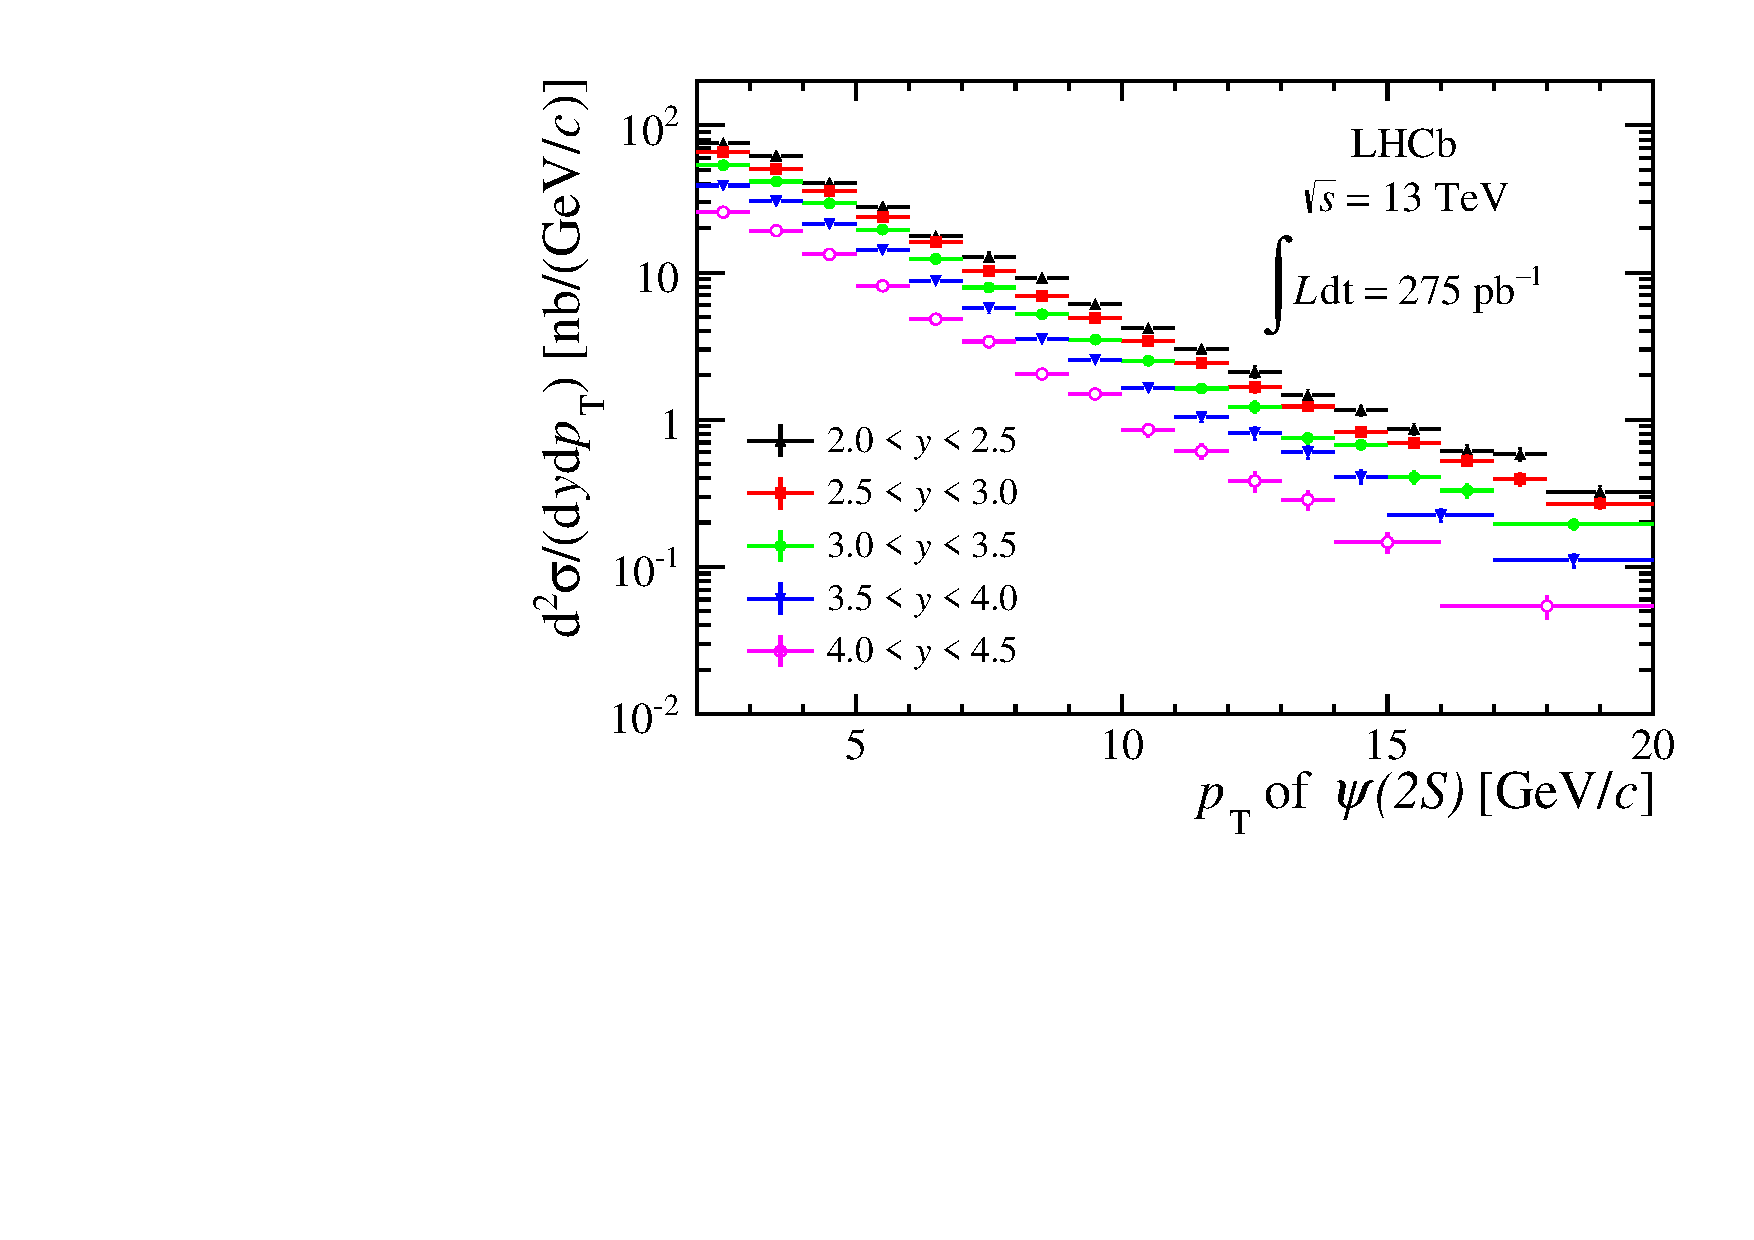
\includegraphics[width=0.9\textwidth]{chap3_result_bdecay}
\caption{来自$b$强子衰变产生的$\psitwos$的双微分产生截面分布图。}
\label{fig:results_fromb}
\end{figure}
%%%%%%%%%%%%%%%%%%%%%%%%%%%%%%%%%%%%%%%%%%%%%%%%%%%%%%%%%%%

通过将双微分截面积分掉$y$,我们可以得到$\pp$对撞直接产生的$\psitwos$与来自$b$强子衰变产生的$\psitwos$随着$\pt$变化的微分截面,如图~\ref{fig:results_PT}所示。
我们将直接产生的$\psitwos$和NRQCD~\cite{Shao:2014yta}的理论计算,来自$b$强子衰变产生的$\psitwos$和fixed-order-plus-next-leading-logarithm (FONLL)~\cite{Cacciari:1998it}的理论计算进行了比较。
通过对比可以发现,在$\pt>7\gevc$的区域,NRQCD计算和实验测量吻合的非常好,FONLL的计算和实验测量在整个区间对的都是挺好的。
如果将双微分截面积分掉$\pt$,我们可以得到$\pp$对撞直接产生的$\psitwos$与来自$b$强子衰变产生的$\psitwos$随着$y$变化的单微分截面,如图~\ref{fig:results_Y}所示。
由于NRQCD在低动量区表述的不好,所以没有提供和实验数据的比较。
基于FONLL的理论计算,与实验数据进行了比较,在误差范围内可以很好的吻合。


%%%%%%%%%%%%%%%%%%%%%%%%%%%%%%%%%%%%%%%%%%%%%%%%%%%%%%%%%%%
\begin{figure}[!tbp]
\centering
\begin{minipage}[t]{0.49\textwidth}
\centering
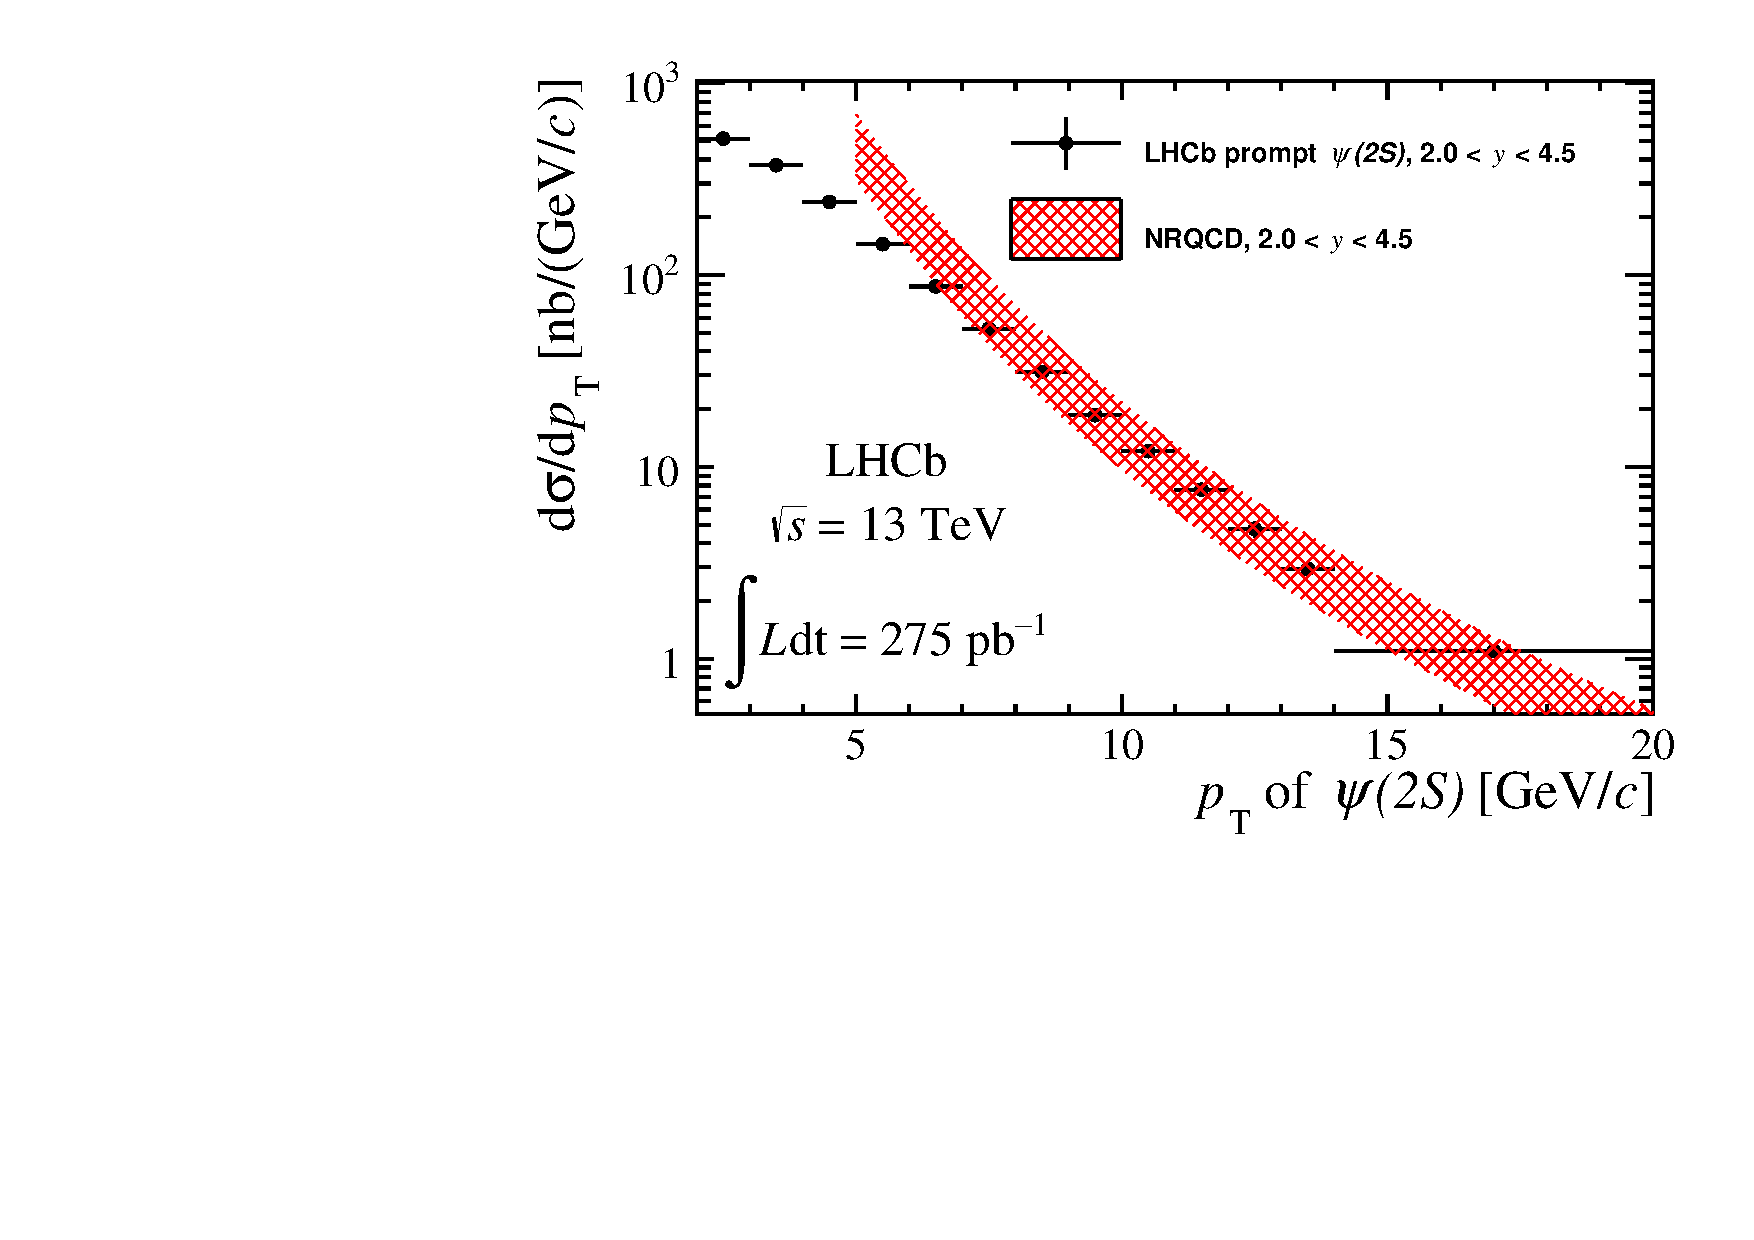
\includegraphics[width=1.0\textwidth]{chap3_PT_result_prompt}
\end{minipage}
\begin{minipage}[t]{0.49\textwidth}
\centering
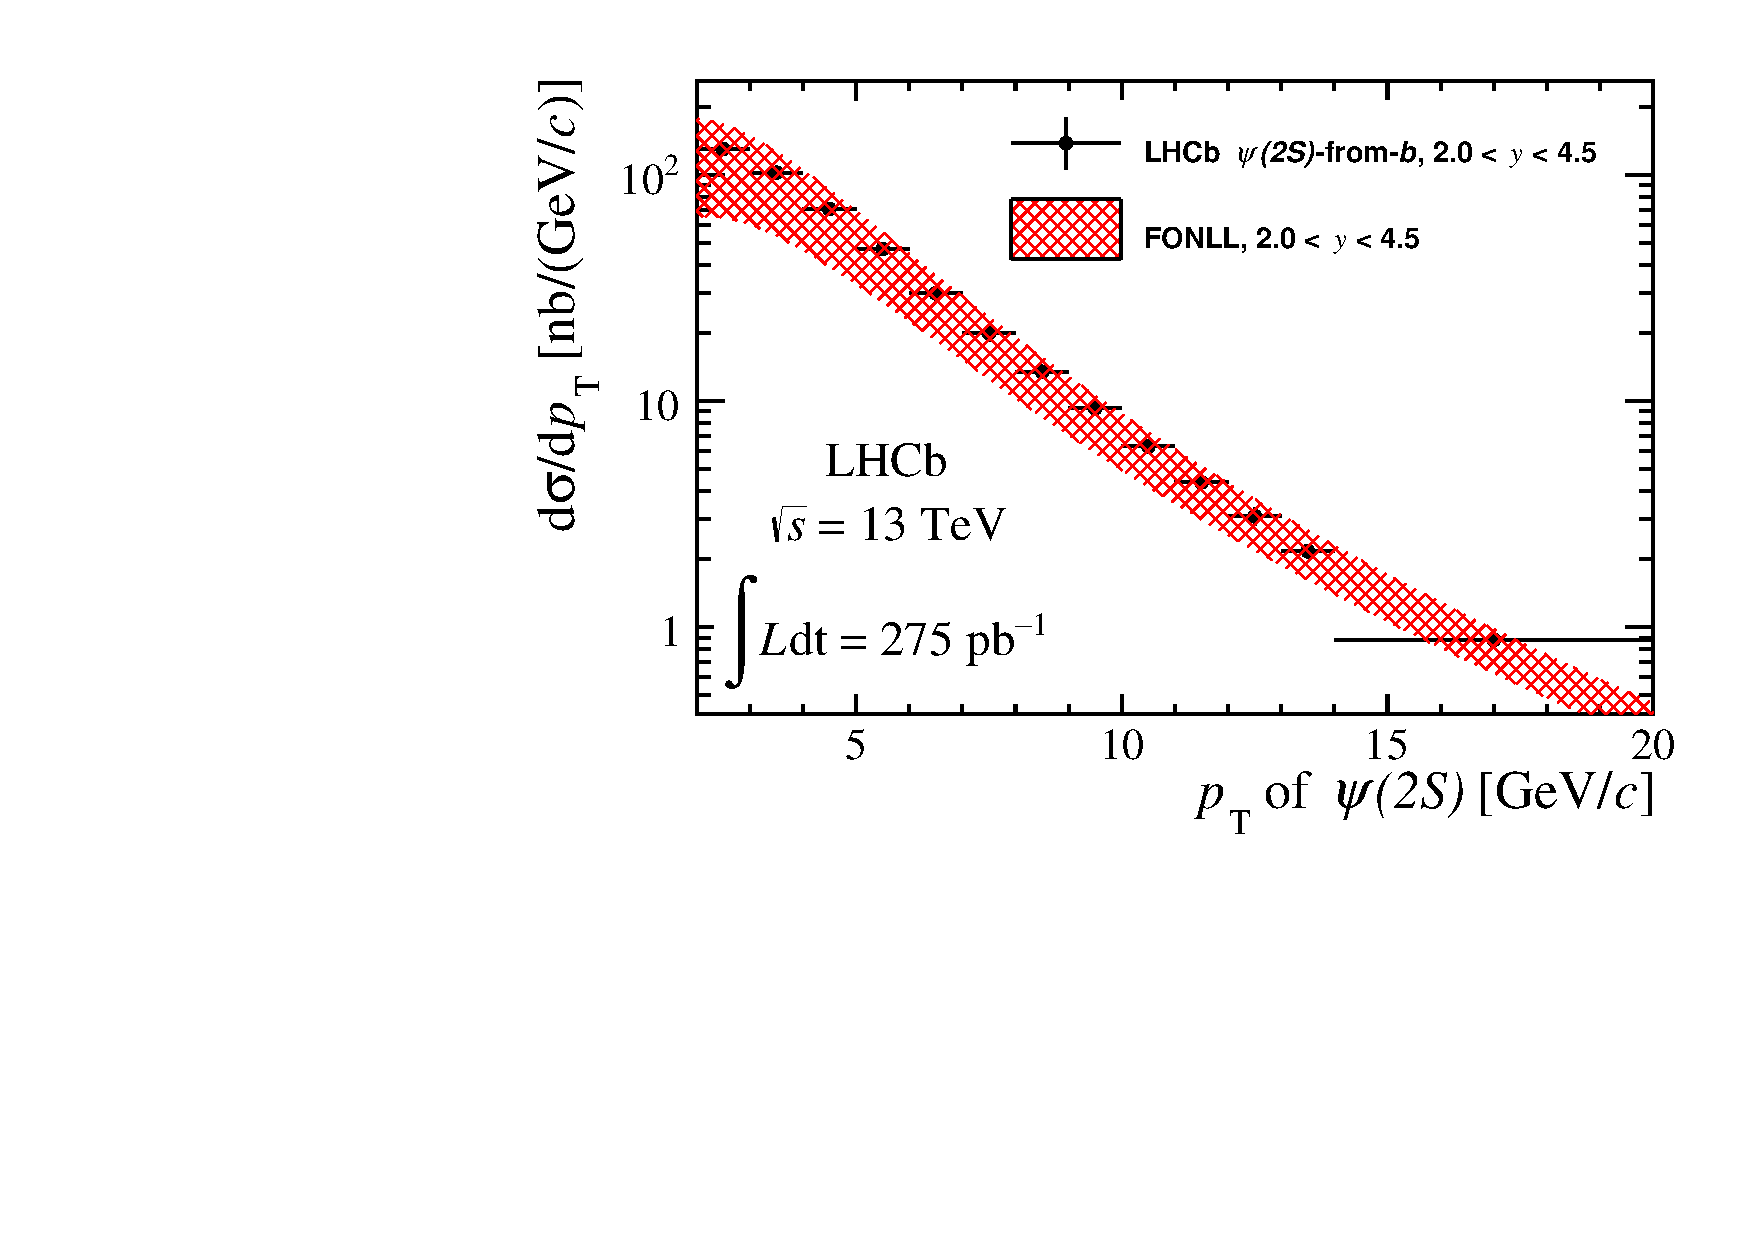
\includegraphics[width=1.0\textwidth]{chap3_PT_result_bdecay}
\end{minipage}
\caption{以$\pt$为函数的(左)$\pp$对撞直接产生的$\psitwos$微分截面与NRQCD计算~\cite{Shao:2014yta}的比较和(右)来自$b$强子衰变产生的$\psitwos$微分截面分布与FONLL~\cite{Cacciari:1998it}的计算比较。}
\label{fig:results_PT}
\end{figure}
%%%%%%%%%%%%%%%%%%%%%%%%%%%%%%%%%%%%%%%%%%%%%%%%%%%%%%%%%%

%%%%%%%%%%%%%%%%%%%%%%%%%%%%%%%%%%%%%%%%%%%%%%%%%%%%%%%%%%%
\begin{figure}[!tbp]
\centering
\begin{minipage}[t]{0.49\textwidth}
\centering
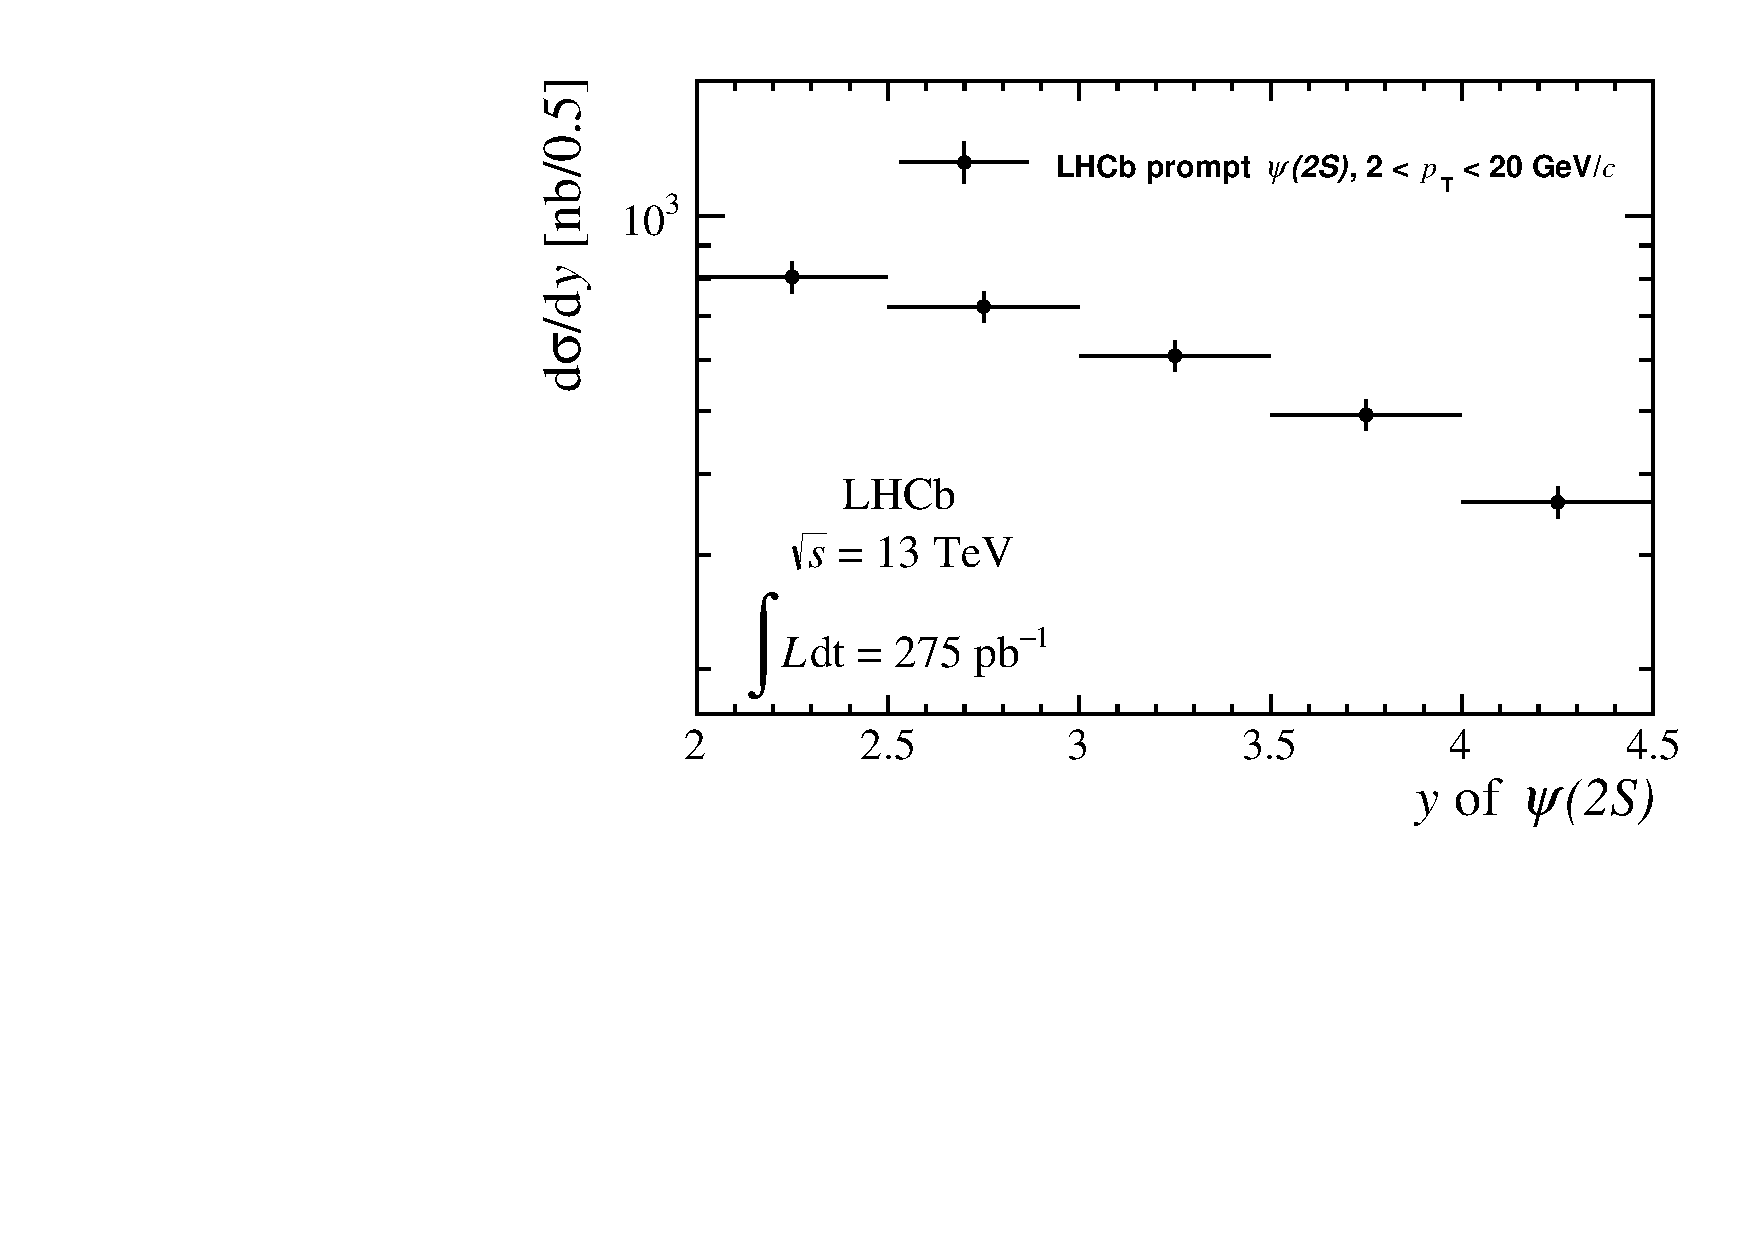
\includegraphics[width=1.0\textwidth]{chap3_Y_result_prompt}
\end{minipage}
\begin{minipage}[t]{0.49\textwidth}
\centering
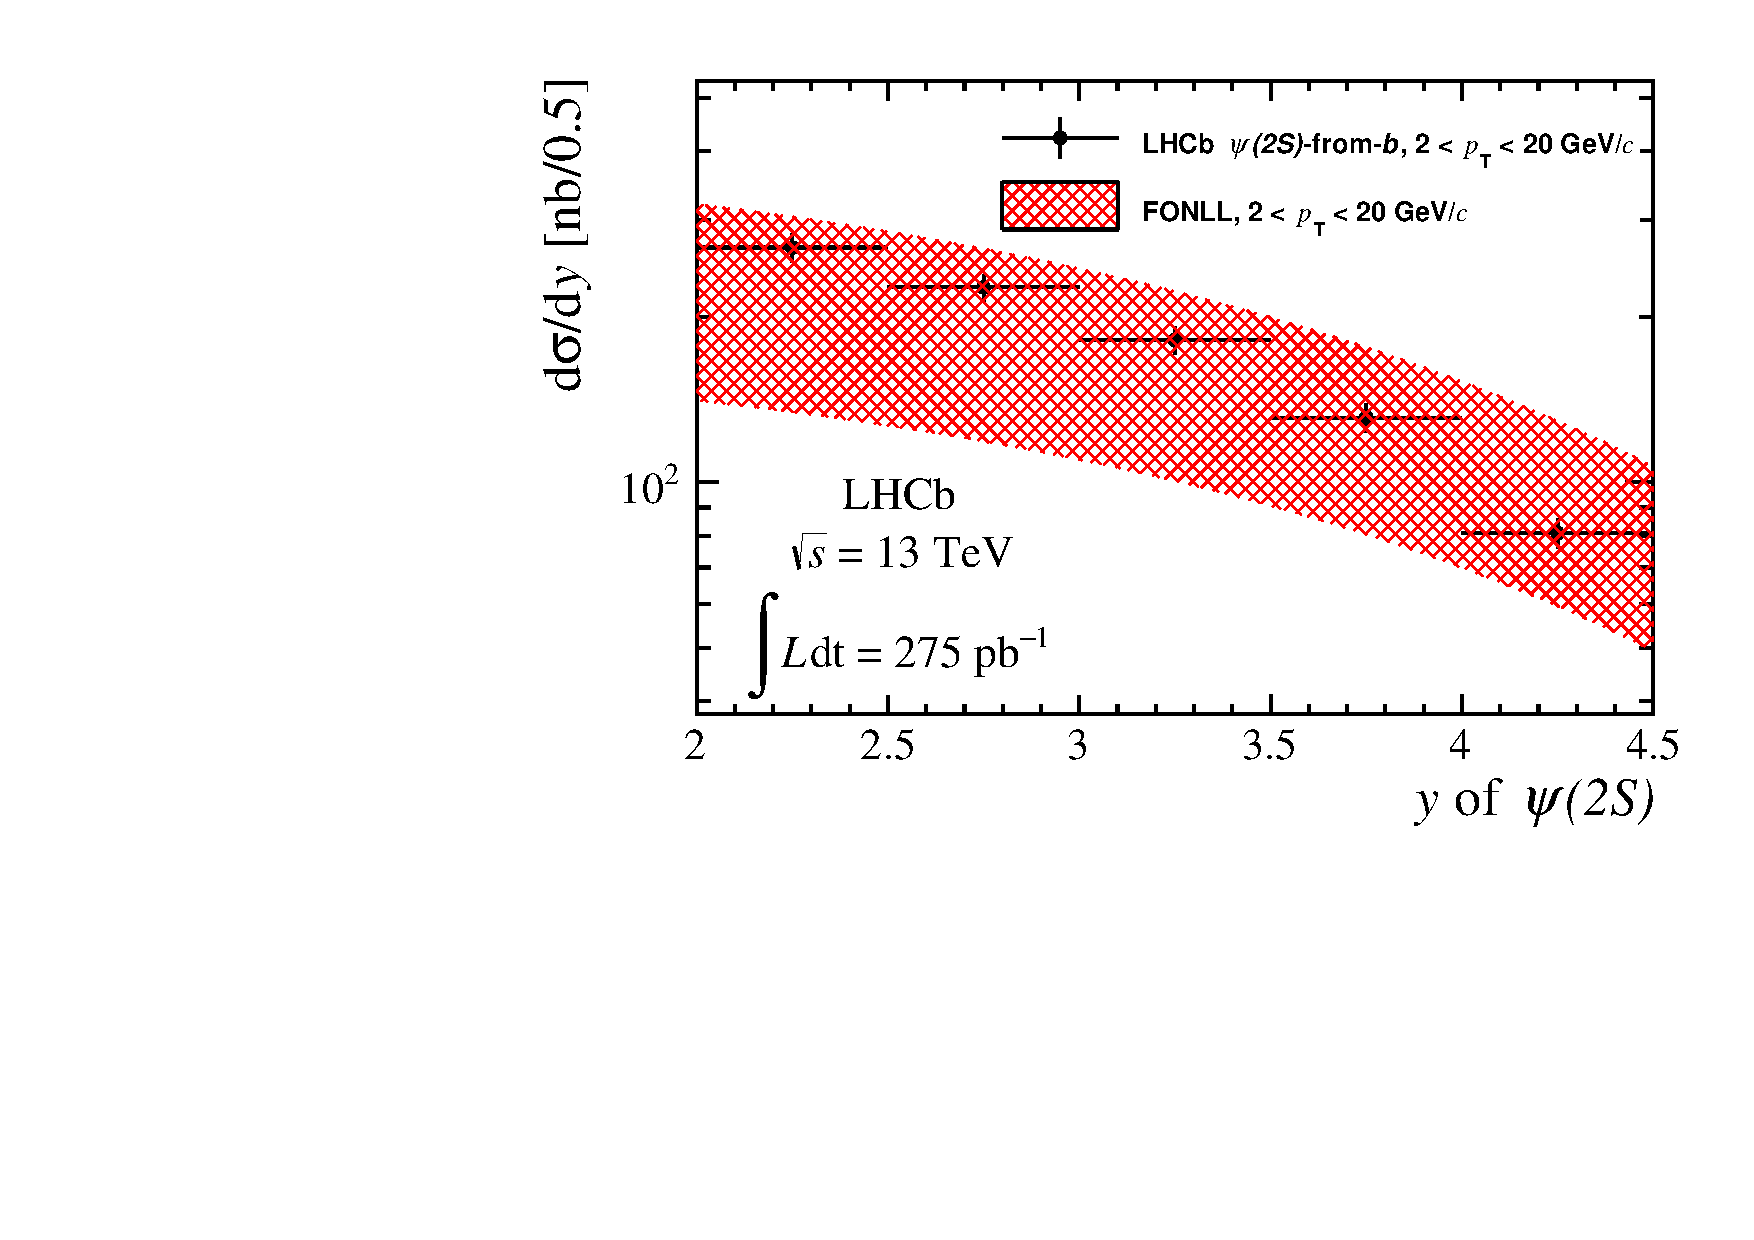
\includegraphics[width=1.0\textwidth]{chap3_Y_result_bdecay}
\end{minipage}
\caption{以$y$为函数的(左)$\pp$对撞直接产生的$\psitwos$微分截面和(右)来自$b$强子衰变产生的$\psitwos$微分截面分布与FONLL~\cite{Cacciari:1998it}的计算比较。}
\label{fig:results_Y}
\end{figure}
%%%%%%%%%%%%%%%%%%%%%%%%%%%%%%%%%%%%%%%%%%%%%%%%%%%%%%%%%%

$\pp$对撞直接产生的$\psitwos$介子和来自$b$强子衰变产生的$\psitwos$介子在运动学范围$\pt$[2,20]、$y$[2,4.5]内的结果如下所示;
\begin{eqnarray*}
\sigma(\mathrm{prompt}~ \psitwos, 2<\pt<20\gevc,2.0<y<4.5) &=& \promptresult,\\
\sigma(\psitwos\text{-from-}\bquark, 2<\pt<20\gevc,2.0<y<4.5) &=& \frombresult,
\end{eqnarray*}
式子中第一个误差是统计误差,第二个误差是系统误差。

\subsection{来自$b$强子衰变产生的$\psitwos$占总$\psitwos$的比例}
\label{sec:Fb}
%%%%%%%%%%%%%%%%%%%%%%%%%%%%%%%%%%%%%%%%%%%%%%%%%%%%%%%%%%%
自$b$强子衰变产生的$\psitwos$占总$\psitwos$的比例, $F_b$,通过每个运动学区间内效率修正之后的直接产生的$\psitwos$的产额, $N_p$,和来自$b$强子衰变产生的$\psitwos$效率修正之后的产额, $N_b$: $F_b=N_b/(N_b+N_p)$.
图~\ref{fig:Fb}给出了比例$F_b$随着$\pt$和$y$的分布。
在每个特定的$y$区间内,比例$F_b$随着$\pt$的增加而增加。
对每个特定的$\pt$区间内,比例$F_b$随着$y$的增加而降低。

%%%%%%%%%%%%%%%%%%%%%%%%%%%%%%%%%%%%%%%%%%%%%%%%%%%%%%%%%%%
\begin{figure}[!tbp]
\centering
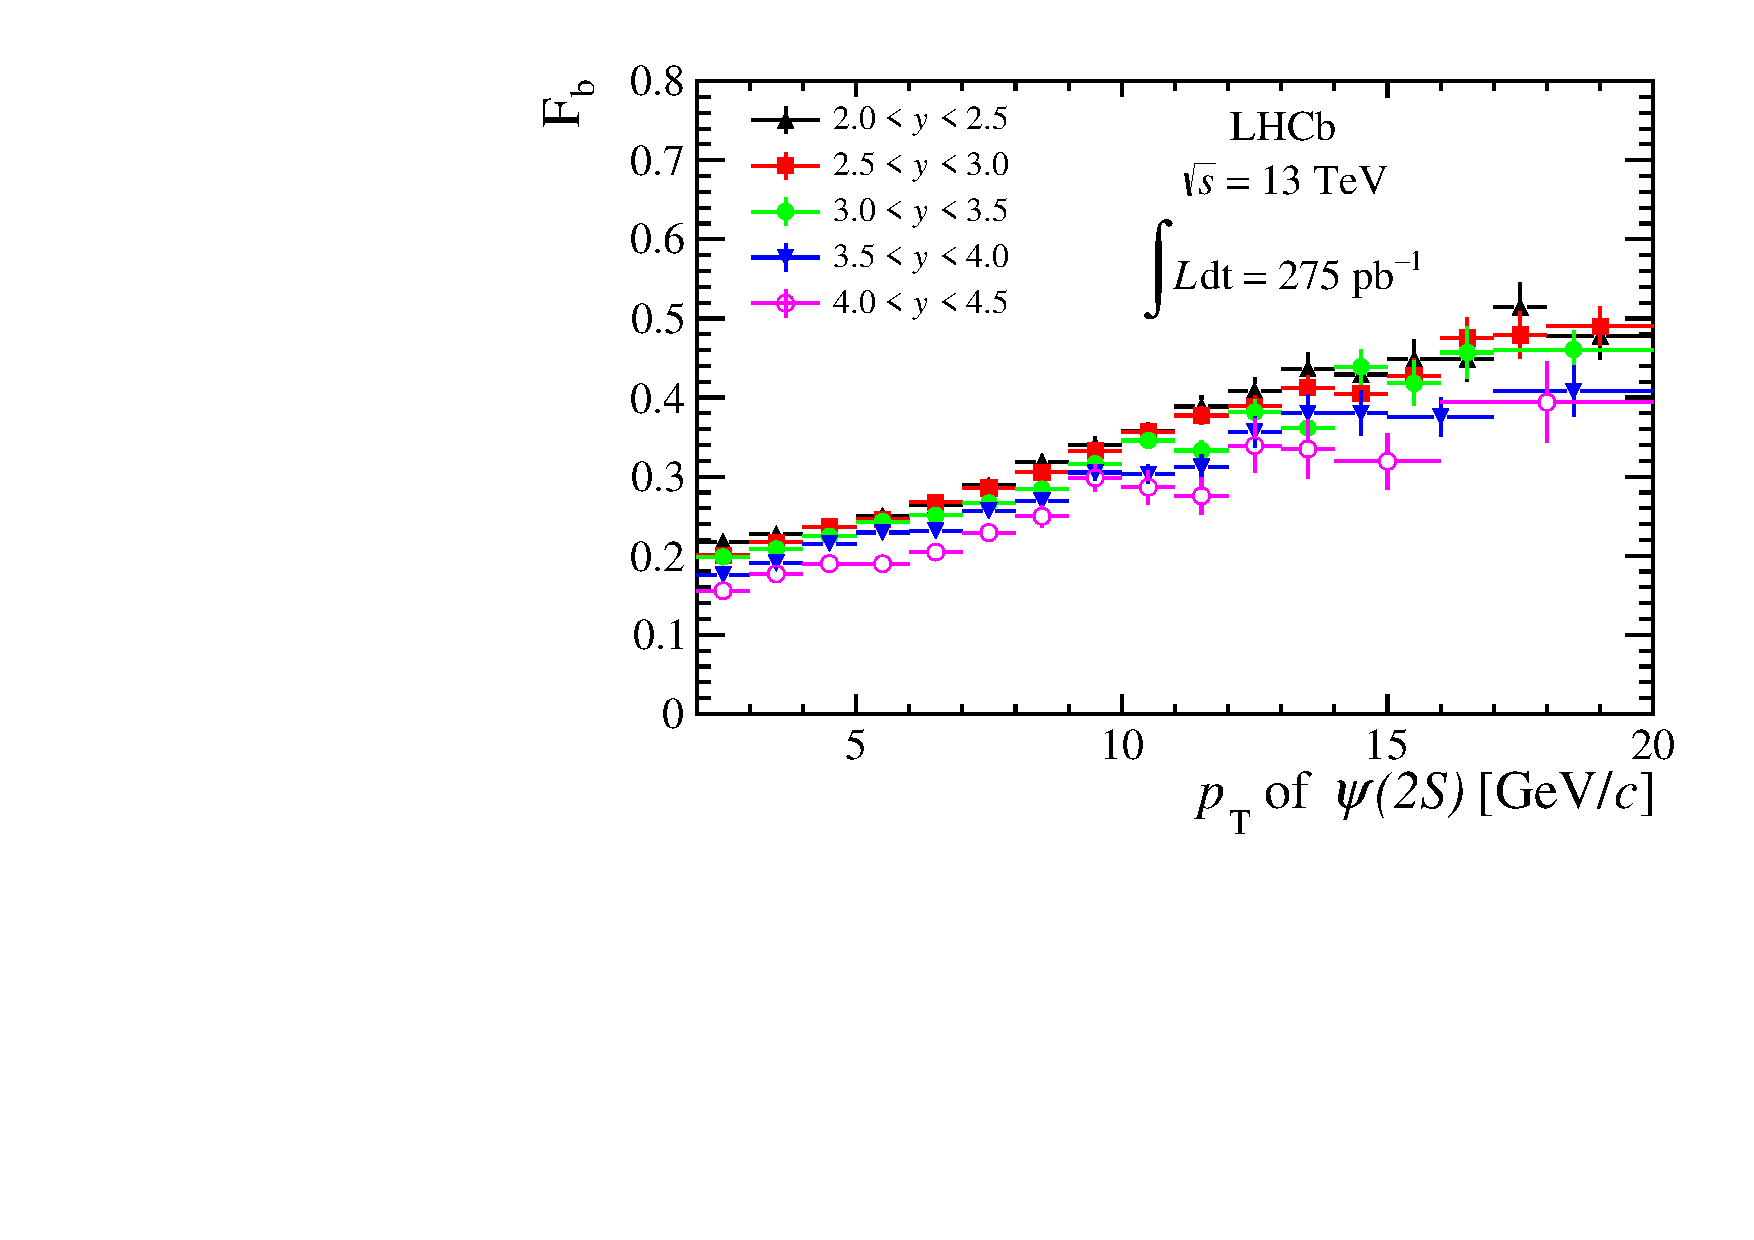
\includegraphics[width=1.0\textwidth]{chap3_Fb}
\caption{$F_b$随着$\pt$和$y$变化的分布。}
\label{fig:Fb}
\end{figure}
%%%%%%%%%%%%%%%%%%%%%%%%%%%%%%%%%%%%%%%%%%%%%%%%%%%%%%%%%%


%%%%%%%%%%%%%%%%%%%%%%%%%%%%%%%%%%%%%%%%%%%%%%%%%%%%%%%%%%
\subsection{拓展到全空间的总$\bbbar$截面}\label{extrapolation}
全空间的总$\bbbar$产生截面通过下面这个公式
\begin{equation}
\sigma(\pp\to\bbbar X) = \alpha_{4 \pi}
\frac{\sigma(\psifromb,\, 2<\pt<20\gevc, \, 2.0 < y < 4.5 )}{2 \mathcal{B}(\bquark\to\psitwos X)}
 \end{equation}
来计算,其中$\alpha_{4 \pi}$ 为修正到4 $\pi$的修正因子,$\bquark\to\psitwos X$的分支比$\mathcal{B}(b \rightarrow \psitwos X) = (2.83 \pm 0.29)\times10^{-3}$~\cite{PDG2017}. 
利用$\lhcb$调试的Pythia 8~\cite{Sjostrand:2007gs}程序, 得到修正因子$\alpha_{4 \pi}=7.29$。
因此,我们得到了$\sqs=13\tev$下总的$\bbbar$产生截面为
\begin{equation*}
\sigma(pp \rightarrow \bquark \bquarkbar X) = 571\pm 3\pm 67\mub,
\end{equation*}
第一项误差为统计误差,第二项为系统误差。分支比$\BF(b \rightarrow \psitwos X)$的误差也已经包含在内。
修正因子$\alpha_{4 \pi }$ 没有考虑误差。
这一结果和$\jpsi$介子的测量结果$\sigma(pp \rightarrow \bquark \bquarkbar X) = 495\pm 2\pm 52\mub$~\cite{LHCb-PAPER-2015-037}在误差范围内是一致的。
如果将我们的结果和$\jpsi$介子的测量结果合并的话,可以给出联合之后的结果$524\pm45\mub$。

\subsection{13 $\tev$下$\psitwos$结果与7 $\tev$下$\psitwos$发表结果的比值}
不同质心能量下微分产生截面比值的研究可以减少系统误差带来的影响,本文对13$\tev$下$\psitwos$微分产生截面和7$\tev$下$\psitwos$微分产生截面报道结果~\cite{LHCb-PAPER-2013-067}的比值$R_{13/7}$进行了研究。
图~\ref{fig:Ratio_7TeV_PT}所示为$R_{13/7}$随着$\pt$变化的分布。
在计算比值$R_{13/7}$的时候,两个分析里面的分支比是按100$\%$完全关联考虑的。
亮度,拟合模型和寻迹效率按照50\%的关联考虑。
其它各项均按照无关考虑。

%%%%%%%%%%%%%%%%%%%%%%%%%%%%%%%%%%%%%%%%%%%%%%%%%%%%%%%%%%%
\begin{figure}[!tbp]
\centering
\begin{minipage}[t]{0.45\textwidth}
\centering
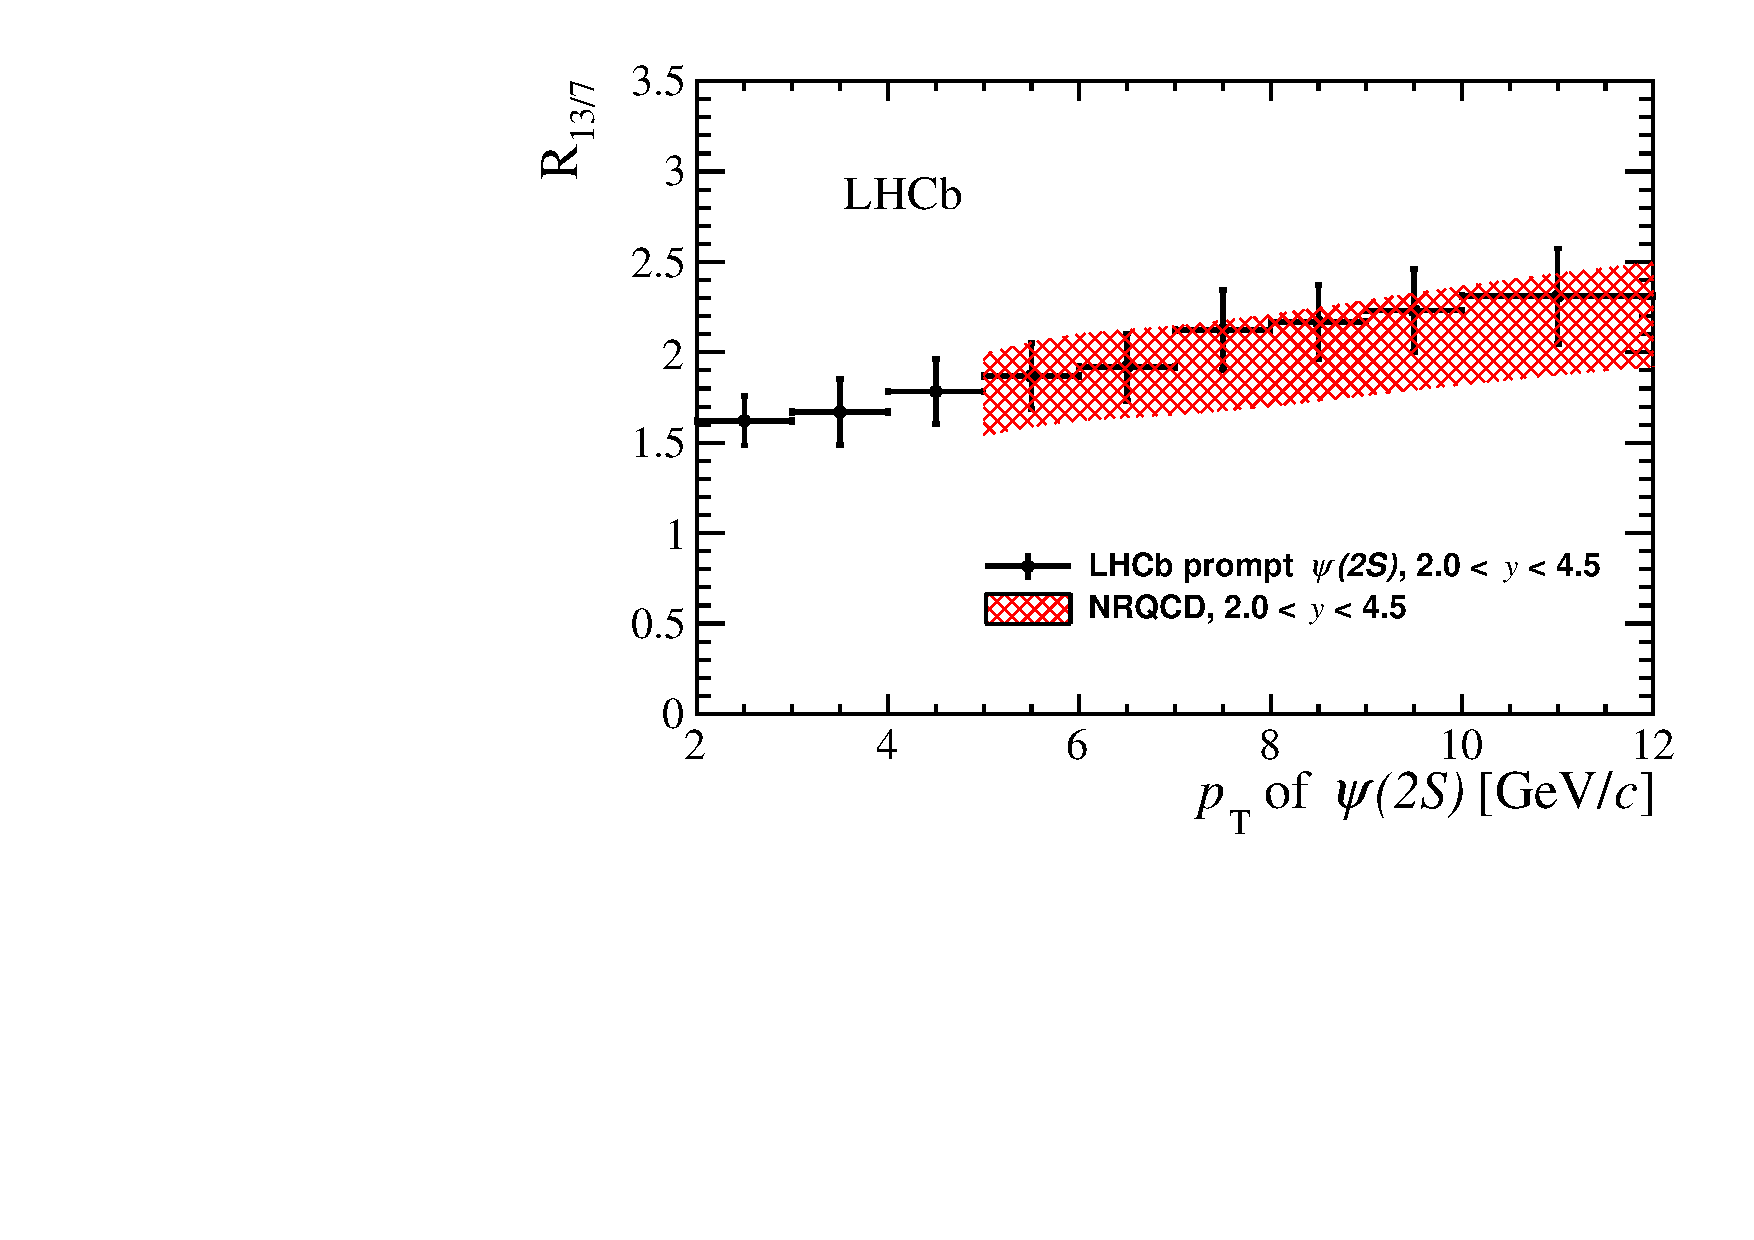
\includegraphics[width=1.0\textwidth]{chap3_Ratio_7TeV_PT_prompt}
\end{minipage}
\begin{minipage}[t]{0.45\textwidth}
\centering
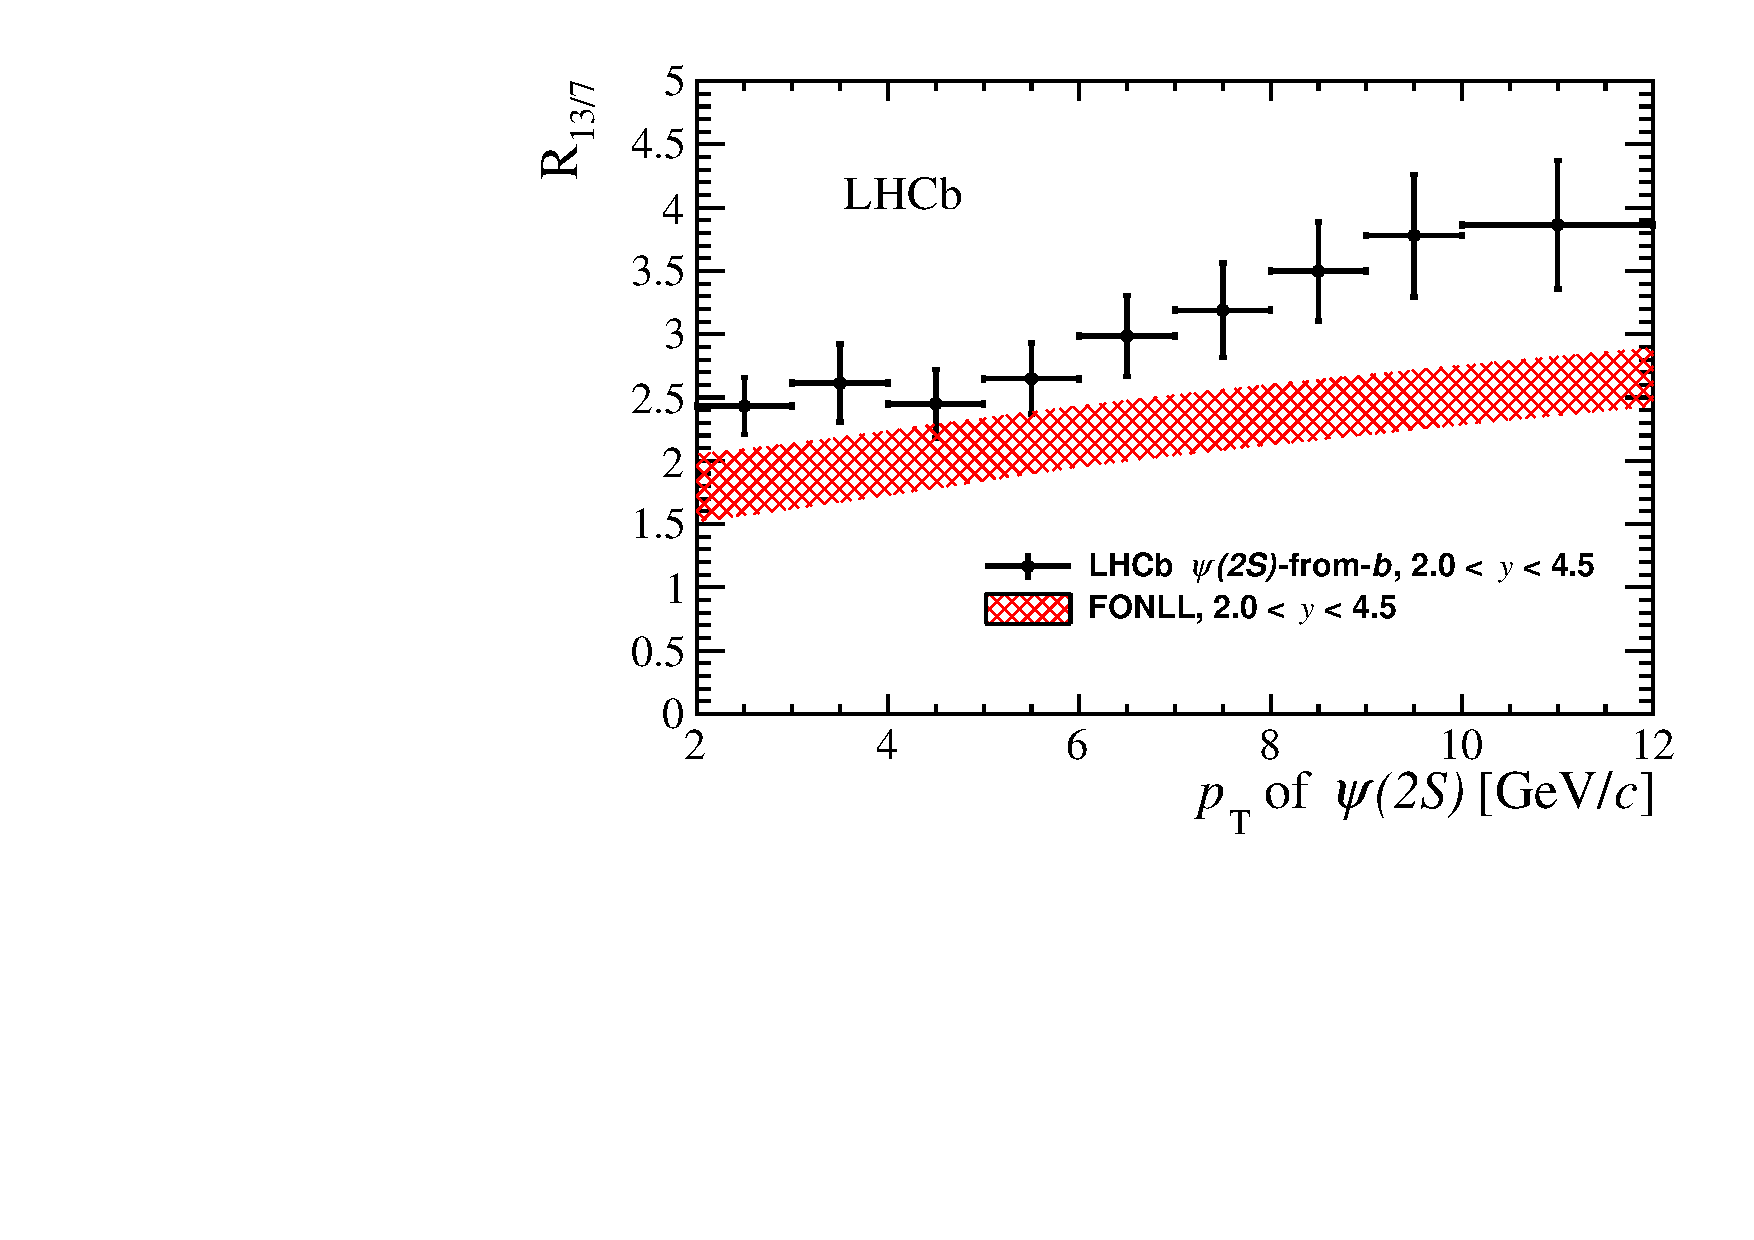
\includegraphics[width=1.0\textwidth]{chap3_Ratio_7TeV_PT_bdecay}
\end{minipage}
\caption{$13\tev$ 与 $7\tev$的产生截面比值随着$\pt$的变化。左图为直接产生的$\psitwos$和NRQCD计算的比较。右图为来自$b$强子衰变产生的$\psitwos$和FONLL的比较。}
\label{fig:Ratio_7TeV_PT}
\end{figure}
%%%%%%%%%%%%%%%%%%%%%%%%%%%%%%%%%%%%%%%%%%%%%%%%%%%%%%%%%%%


\subsection{13 $\tev$下$\psitwos$结果与13 $\tev$下$\jpsi$发表结果的比值}
我们对13 $\tev$下$\psitwos$微分产生截面和13 $\tev$下$\jpsi$微分产生截面~\cite{LHCb-PAPER-2015-037}($0<\pt<14\gevc$,$2.0<y<4.5$)的比值$\Rpsijpsi$进行了研究。
如图~\ref{fig:Ratio_jpsi_PT_prompt} 所示为对于$\pp$对撞直接产生的$\psitwos$与$\jpsi$的截面比值。
左(右)图展示了$\Rpsijpsi$对于积分掉$2<y<4.5$($2<\pt<14$)之后随着$\pt$($y$)变化的分布。
左图同时提供了NRQCD的理论计算作为比较。
图~\ref{fig:Ratio_jpsi_PT_bdecay} 所示为来自$b$强子衰变产生的$\psitwos$与$\jpsi$的截面比值。
左(右)图展示了$\Rpsijpsi$对于积分掉$2<y<4.5$($2<\pt<14$)之后随着$\pt$($y$)变化的分布。
同时提供了FONLL的理论计算作为比较。
为了计算两个截面测量之间的比值,二者之间的亮度,径迹重建,拟合模型系统误差是按照完全关联处理的。
其它的误差都假定为完全无关。

%%%%%%%%%%%%%%%%%%%%%%%%%%%%%%%%%%%%%%%%%%%%%%%%%%%%%%%%%%%
\begin{figure}[!tbp]
\centering
\begin{minipage}[t]{0.45\textwidth}
\centering
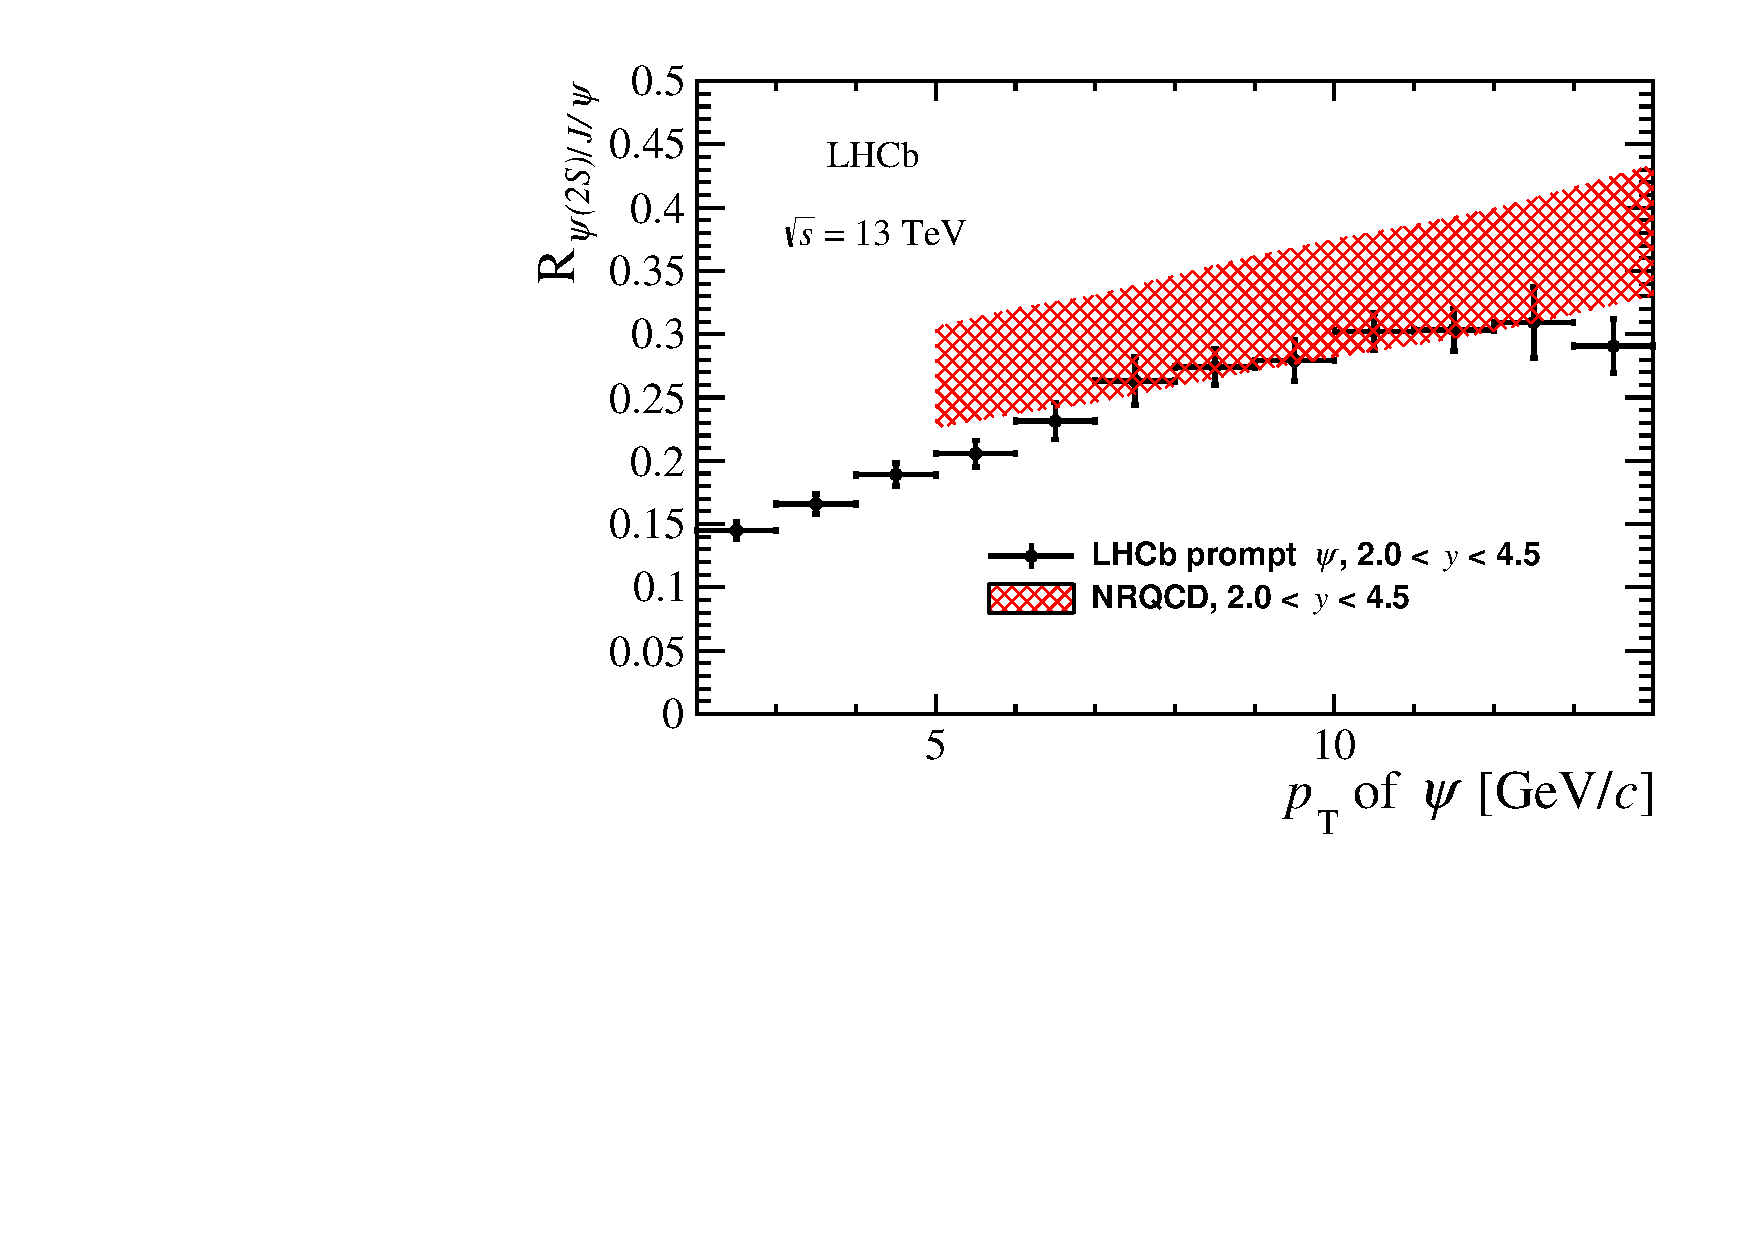
\includegraphics[width=1.0\textwidth]{chap3_Ratio_jpsi_PT_prompt}
\end{minipage}
\begin{minipage}[t]{0.45\textwidth}
\centering
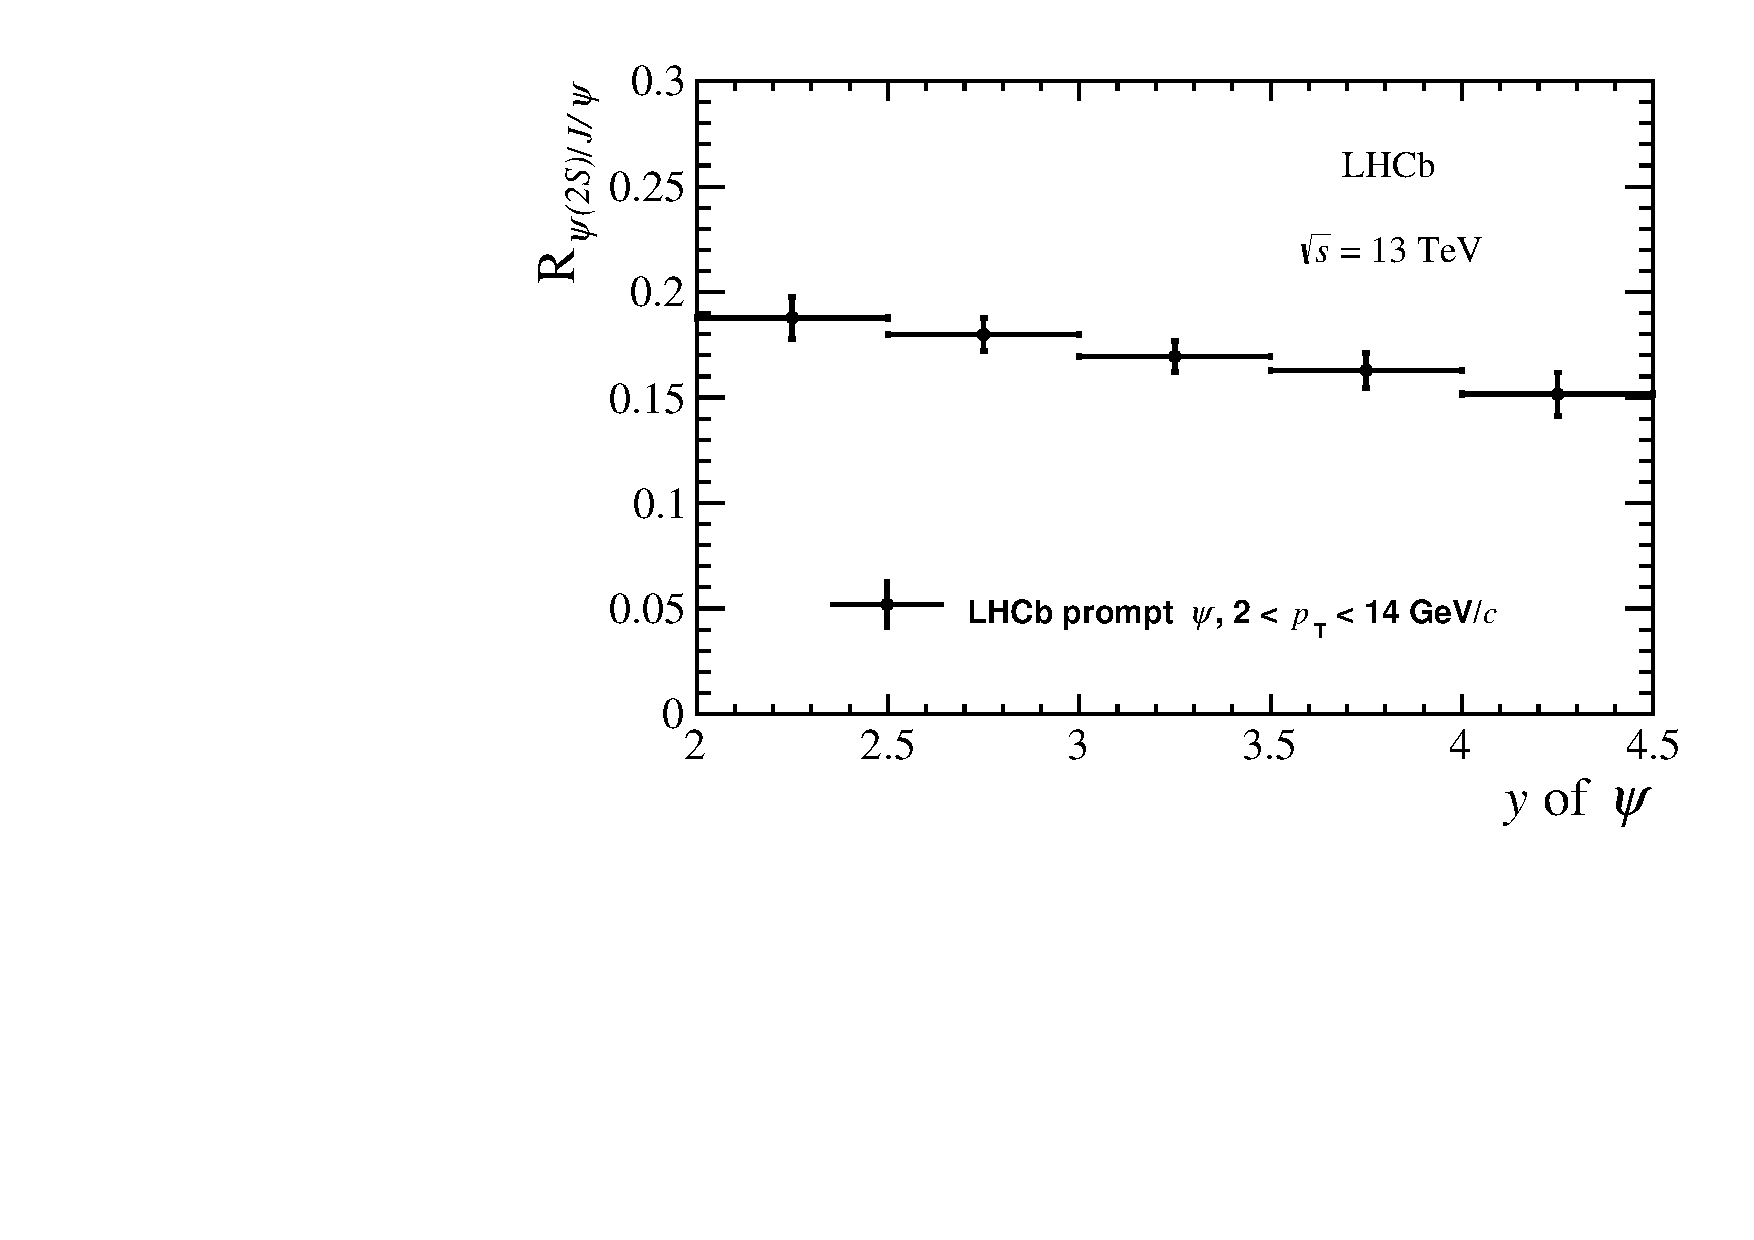
\includegraphics[width=1.0\textwidth]{chap3_Ratio_jpsi_Y_prompt}
\end{minipage}
\caption{$\pp$对撞直接产生的$\psitwos$与13$\tev$下$\jpsi$发表结果的比值随着$\pt$(左图)和$y$(右图)的变化图。}
\label{fig:Ratio_jpsi_PT_prompt}
\end{figure}
%%%%%%%%%%%%%%%%%%%%%%%%%%%%%%%%%%%%%%%%%%%%%%%%%%%%%%%%%%%
\begin{figure}[!tbp]
\centering
\begin{minipage}[t]{0.45\textwidth}
\centering
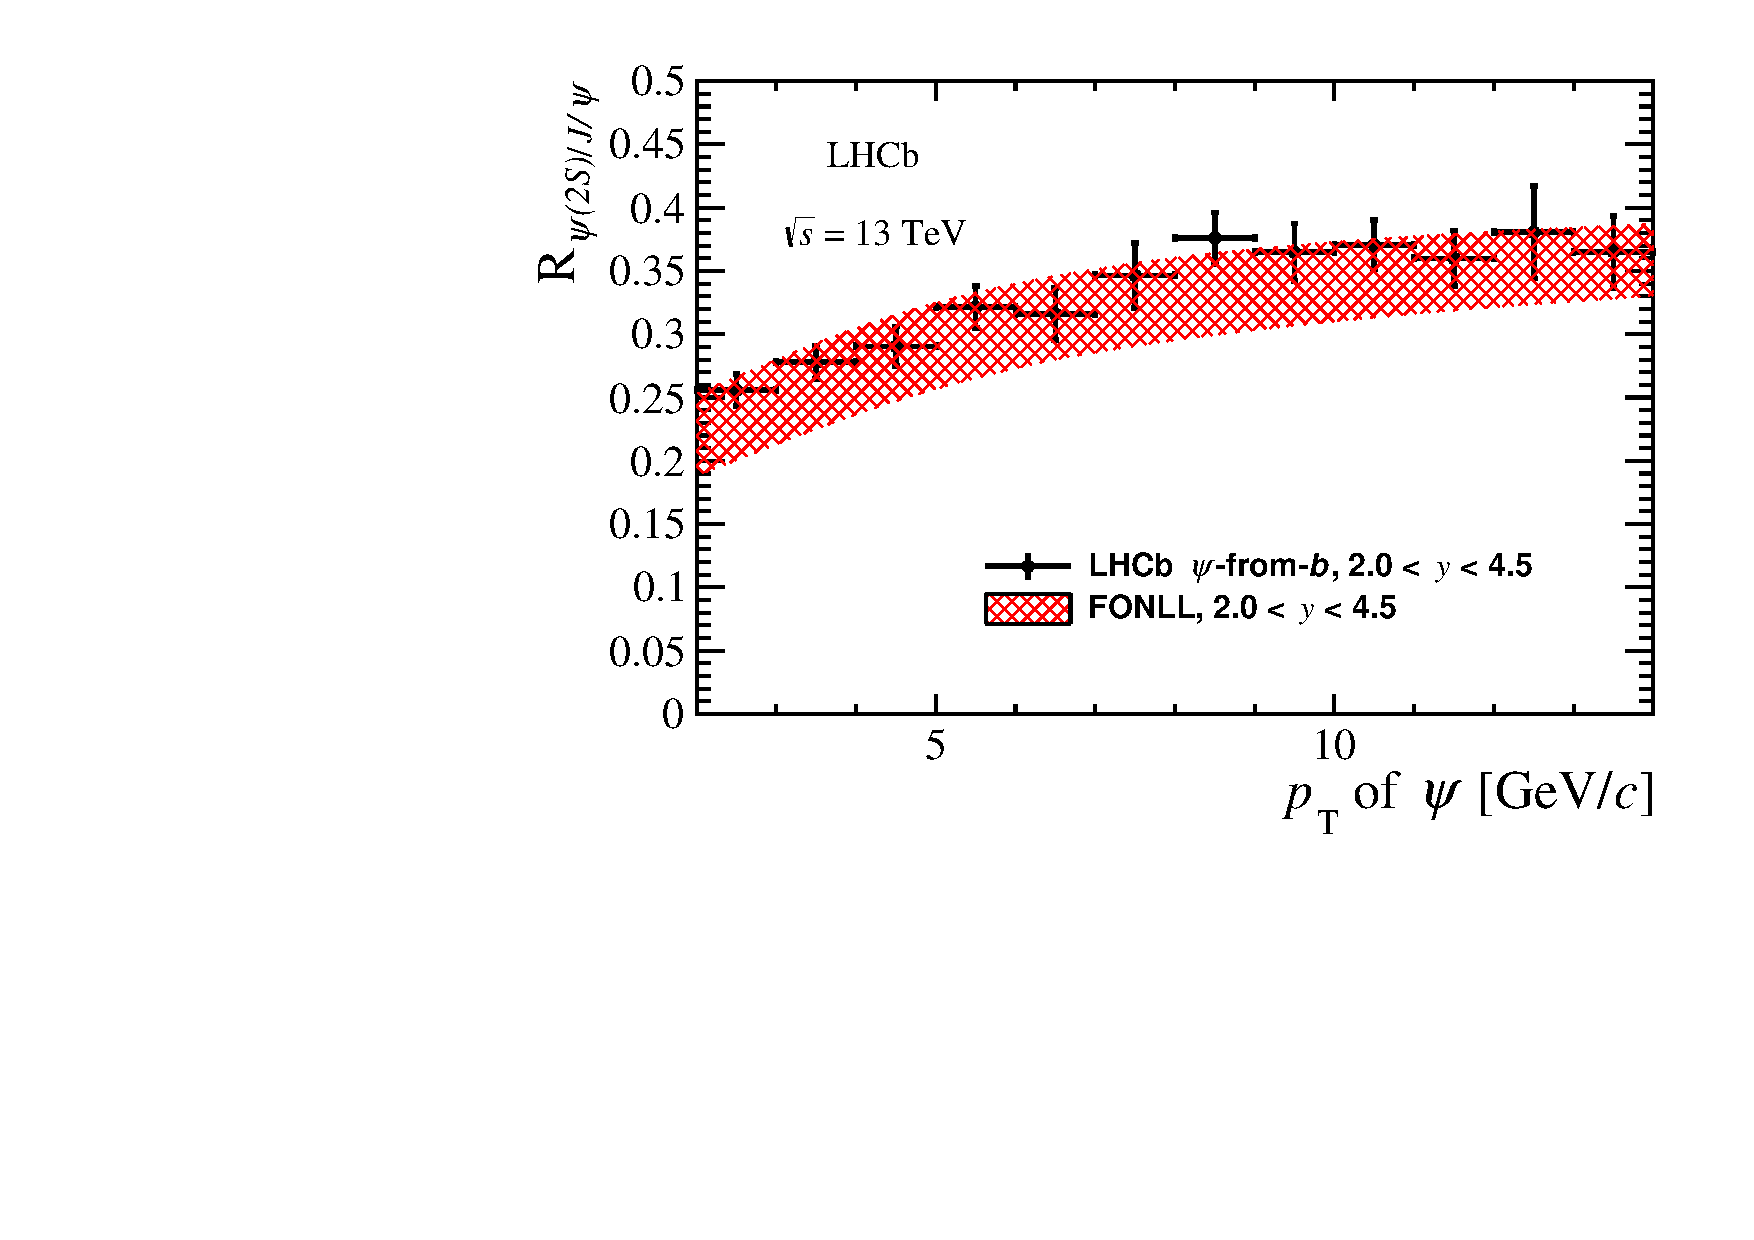
\includegraphics[width=1.0\textwidth]{chap3_Ratio_jpsi_PT_bdecay}
\end{minipage}
\begin{minipage}[t]{0.45\textwidth}
\centering
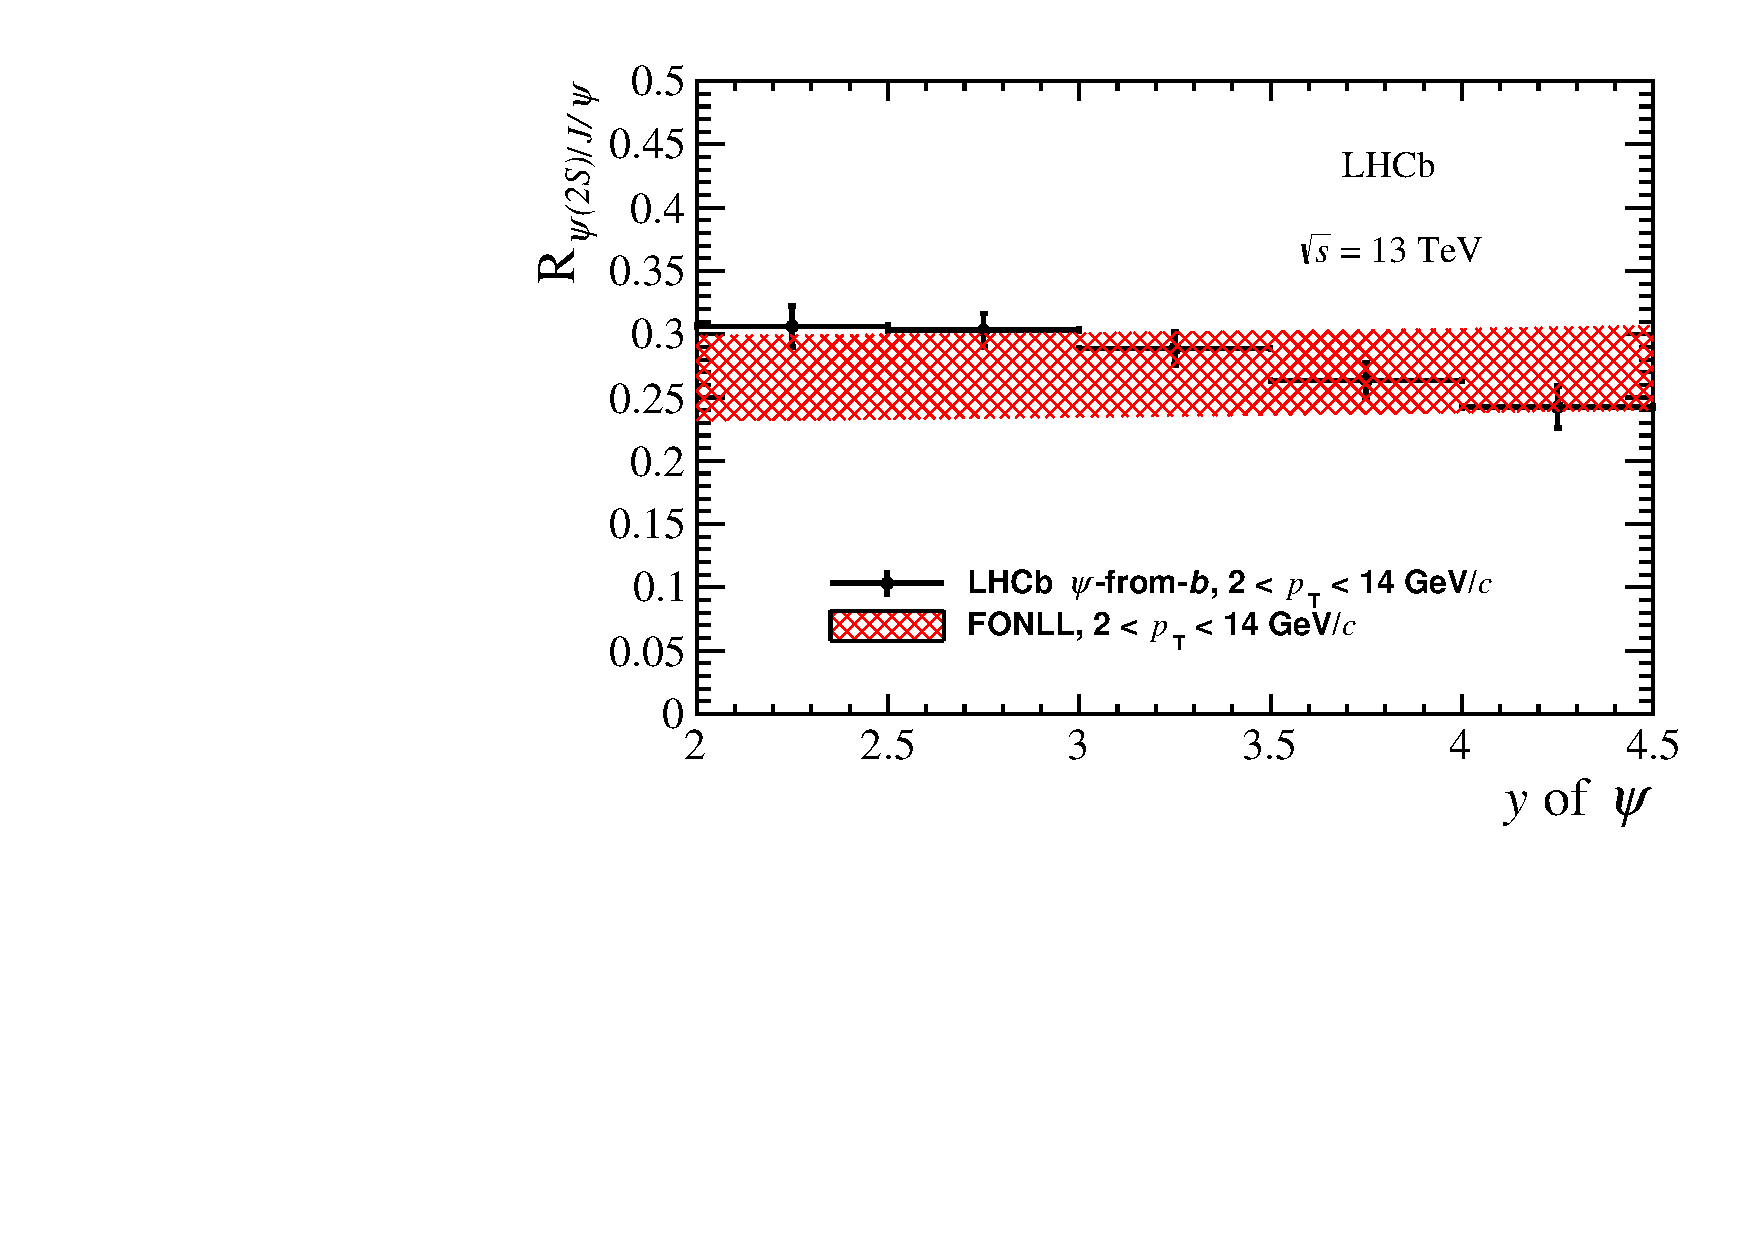
\includegraphics[width=1.0\textwidth]{chap3_Ratio_jpsi_Y_bdecay}
\end{minipage}
\caption{$b$强子衰变而来的$\psitwos$与13$\tev$下$\jpsi$发表结果的比值随着$\pt$(左图)和$y$(右图)的变化图。}
\label{fig:Ratio_jpsi_PT_bdecay}
\end{figure}
%%%%%%%%%%%%%%%%%%%%%%%%%%%%%%%%%%%%%%%%%%%%%%%%%%%%%%%%%%%


\subsection{小节}
本章主要讲了13 $\tev$下$\psitwos$微分截面测量,并给出了微分截面测量结果。
测量结果与7 $\tev$下$\psitwos$发表结果的比值,和与13 $\tev$下$\jpsi$发表结果的比值。


